\documentclass[UTF8,a4paper,11pt]{ctexart}
\usepackage[margin=2.2cm]{geometry}
\usepackage{amsmath,amssymb,booktabs,graphicx,hyperref,xcolor}
\usepackage{float}
\hypersetup{colorlinks=true,linkcolor=blue,urlcolor=blue}
\graphicspath{{../../../units/task2_classification/results/figures/stage2/}{../../../units/task2_classification/results/figures/}}
\setlength{\parindent}{2em}
\setlength{\parskip}{0.35em}
\title{Task2：AG-News 分类模型设计、对比与分析}
\author{DL Foundations Lab}
\date{2026.06.22 -- 2026.06.28}

\begin{document}
\maketitle

\begin{abstract}
本任务围绕简单分类模型设计与实现，选择 AG-News 文本分类数据集进行实验。AG-News 数据规模适中、训练成本较低，因此用于完整比较 MLP/FN、FastText-style pooling、TextCNN、LSTM/BiLSTM、BiLSTM-Attention、RCNN、TransformerEncoder 与 DistilBERT。所有配置选择均基于 validation set，test set 仅作为最终观察。本轮结果显示，AG-News 上轻量 scratch 模型大多处于 91\%--92\% test accuracy 区间，DistilBERT fine-tuning 达到 94.66\% test accuracy；概率平均 ensemble 达到 93.92\% test accuracy，作为有效的模型互补性验证保留。
\end{abstract}

\section{任务目标与研究问题}
研究问题如下：RQ1，轻量模型是否能在 AG-News 上接近或超过参考 baseline；RQ2，更强文本结构、预训练表示和 ensemble 是否带来稳定收益；RQ3，scratch 模型的结构、训练成本和泛化行为有何差异；RQ4，validation 选择与 test observation 是否一致；RQ5，错误主要集中在哪些类别。

\section{数据集与实验协议}
\subsection{AG-News}
AG-News 使用 Hugging Face \texttt{ag\_news}。官方 train/test 为 120000/7600；本实验从官方 train split 中按 label 分层切出 10\% validation，seed=42，最终为 train=108000、validation=12000、test=7600。标签为 0 World、1 Sports、2 Business、3 Sci/Tech。

文本预处理采用 lowercase regex tokenizer，词表仅由 train split 构建，\texttt{<pad>}=0，\texttt{<unk>}=1。轻量模型默认 \texttt{vocab\_size}=30000、\texttt{max\_seq\_len}=128；强化实验按配置扩展到 50000 词表或 256 长度。LSTM 系列通过 \texttt{pack\_padded\_sequence} 避免 padding 位置污染序列状态。

\section{模型设计与实现}
\subsection{文本模型}
MLP/FN 使用 masked mean pooling 后接两层全连接，用于验证主题词信号的强度。FastText-style 模型保留均值池化思路，但使用更大的 embedding 表达浅层 n-gram/词汇信号。TextCNN 使用多 kernel 卷积：
\[
h_k=\mathrm{ReLU}(\mathrm{Conv1d}_k(X)), \quad z_k=\max_t h_{k,t}, \quad y=W[z_2,z_3,z_4,z_5]+b .
\]
LSTM/BiLSTM 使用门控序列状态；BiLSTM-Attention 对所有有效位置学习 attention 权重。RCNN 拼接 embedding 与 BiLSTM 上下文后做 max pooling。TransformerEncoder 从零训练两层自注意力编码器，用于检验“无预训练自注意力”是否优于 TextCNN。DistilBERT fine-tuning 使用预训练 \texttt{distilbert-base-uncased}，只提交指标和预测，不提交模型权重。

\section{正确性验证与工程检查}
\begin{table}[H]
\centering
\caption{AG-News correctness checks}
\begin{tabular}{ll}
\toprule
检查项 & 结果 \\
\midrule
split 数量与 label set & passed \\
tokenizer / label mapping & passed \\
padding / length mask & passed \\
single batch loss & 1.7984 $\rightarrow$ 0.0007 \\
train/eval dropout mode & passed \\
\bottomrule
\end{tabular}
\end{table}

工程层面保留数据与 checkpoint 的忽略规则，AG-News CSV、HF cache、模型权重均不提交。DistilBERT 下载时出现 Windows symlink 降级提示，但不影响模型加载和 fine-tuning。

\section{AG-News 轻量基线实验}
\subsection{轻量基线实验设置}
AG-News 轻量基线实验用于建立从零训练模型的可解释参照。所有轻量模型共享相同数据划分：官方 train split 中按 label 分层切出 10\% 作为 validation，seed=42；test set 仅用于最终 observation。文本侧统一使用 lowercase regex tokenizer，词表仅由 train split 构建，\texttt{<pad>}=0、\texttt{<unk>}=1。除特别说明外，轻量模型使用 \texttt{vocab\_size}=30000、\texttt{max\_seq\_len}=128、\texttt{batch\_size}=128、Adam 优化器、\texttt{learning\_rate}=1e-3、\texttt{weight\_decay}=1e-4 和 6 epoch 快速筛选预算。训练目标为 cross entropy；配置选择标准为 validation accuracy，test set 只用于最终 observation。

\begin{table}[H]
\centering
\caption{AG-News lightweight suite 模型与用途}
\small
\begin{tabular}{llll}
\toprule
run & model & structure & purpose \\
\midrule
baseline\_textcnn & TextCNN & Embedding + Conv1D + max pooling & TextCNN baseline \\
hparam\_dropout\_0.2 & TextCNN & same as baseline & regularization strength \\
model\_mlp & MLP/FN & masked mean pooling + 2-layer MLP & word-level topic signal \\
model\_bilstm & BiLSTM & packed bidirectional LSTM & sequence context \\
\bottomrule
\end{tabular}
\end{table}

\begin{table}[H]
\centering
\caption{AG-News lightweight suite 训练配置}
\small
\begin{tabular}{lcccccc}
\toprule
run & emb & hidden/filters & dropout & optimizer & lr & epochs \\
\midrule
baseline\_textcnn & 128 & filters=128 & 0.5 & Adam & 1e-3 & 6 \\
hparam\_dropout\_0.2 & 128 & filters=128 & 0.2 & Adam & 1e-3 & 6 \\
model\_mlp & 128 & hidden=256 & 0.5 & Adam & 1e-3 & 6 \\
model\_bilstm & 128 & hidden=128 & 0.5 & Adam, clip=5.0 & 1e-3 & 6 \\
\bottomrule
\end{tabular}
\end{table}

TextCNN 的计算形式为
\[
h_k = \mathrm{ReLU}(\mathrm{Conv1D}_k(X)), \quad
z_k = \max_t h_{k,t}, \quad
\hat{y}=W[z_3,z_4,z_5]+b.
\]
不同 kernel size 分别捕捉不同长度的局部 n-gram 模式。MLP/FN 对非 padding token 的 embedding 做 masked mean pooling，作为最简单的词级主题聚合模型。BiLSTM 通过双向门控状态建模上下文，并用 \texttt{pack\_padded\_sequence} 避免 padding 位置污染序列状态。

\subsection{轻量基线结果}
\begin{table}[H]
\centering
\caption{AG-News lightweight suite 摘要}
\begin{tabular}{lcccc}
\toprule
run & model & best epoch & best val acc & test acc \\
\midrule
baseline\_textcnn & TextCNN & 6 & 0.9192 & 0.9149 \\
hparam\_dropout\_0.2 & TextCNN & 6 & 0.9228 & 0.9167 \\
model\_mlp & MLP & 6 & 0.9198 & 0.9121 \\
model\_bilstm & BiLSTM & 5 & 0.9183 & 0.9163 \\
\bottomrule
\end{tabular}
\end{table}

轻量实验的主要结论不是某个 scratch 模型已经充分优化，而是 AG-News 存在较强主题词信号：MLP/FN 通过均值池化已接近 TextCNN，说明很多样本可以由词级主题特征区分。TextCNN 在 validation 上略优，说明局部短语模式仍有价值；BiLSTM 的 test observation 接近 TextCNN，但 validation 未形成稳定优势，说明在 6 epoch 预算下序列模型尚未充分体现其上下文建模能力。

每个 epoch 的 \texttt{train\_loss}、\texttt{train\_acc}、\texttt{val\_loss}、\texttt{val\_acc} 和 \texttt{val\_macro\_f1} 已保存到各 run 的 \texttt{metrics.csv}。例如 \texttt{baseline\_textcnn} 的 validation accuracy 从 epoch 1 的 0.8653 上升到 epoch 6 的 0.9192，\texttt{hparam\_dropout\_0.2} 从 0.8732 上升到 0.9228；对应训练曲线用于检查训练是否持续收敛、是否出现明显过拟合以及最佳 epoch 是否发生在训练末端。

最优 lightweight validation run 是 \texttt{hparam\_dropout\_0.2}，其 test observation 为 0.9167，尚未稳定超过 92\%。由于该 run 在第 6 epoch 仍达到最佳 validation，6 epoch 更适合作为快速筛选预算，而不是最终训练上限。后续强化实验因此不再只做小范围调参，而是从训练预算、训练策略、模型结构和预训练表示四个方向继续验证。

\begin{figure}[H]
\centering

\includegraphics[width=0.78\textwidth]{hparam_val_acc_comparison.png}
\caption{AG-News lightweight validation accuracy, zoomed scale. The x-axis is truncated to 0.88--0.93 to show small validation differences.}
\end{figure}

图中横轴采用缩放范围，而不是默认 0--1 accuracy 范围，因此可以看出 \texttt{hparam\_dropout\_0.2} 相比 baseline 和其他轻量模型的细微优势。红色参考线表示 92\% validation reference。该图只能说明同一 AG-News lightweight suite 内部的 validation 差异，不能把 0.1\%--0.3\% 的视觉差异解释为稳定统计优势；最终仍需要结合 test observation 和训练曲线。

\section{AG-News 强化实验}
\subsection{强化实验设置}
强化实验的目标是验证轻量 scratch 模型未稳定超过 92\% 的原因：是训练预算不足、训练策略不足、模型结构表达不足，还是缺少预训练语言知识。为避免把多种因素混在一起解释，本节将强化实验分为四类：训练策略增强、scratch 架构增强、预训练模型 fine-tuning 和概率平均 ensemble。

\begin{table}[H]
\centering
\caption{AG-News strengthened suite 模型与改进点}
\small
\begin{tabular}{llll}
\toprule
label & model & source & improvement point \\
\midrule
TextCNN+LS & TextCNN & scratch & label smoothing reduces over-confidence \\
BiLSTM20 & BiLSTM & scratch & longer sequence-model training budget \\
FastText-style & lexical pooling & scratch & shallow lexical pooling signal \\
Transformer-s & TransformerEncoder & scratch & self-attention without pretraining \\
DistilBERT & DistilBERT & pretrained & contextual representation transfer \\
Ensemble & Probability average & no retraining & model complementarity \\
\bottomrule
\end{tabular}
\end{table}

\begin{table}[H]
\centering
\caption{AG-News strengthened suite 训练配置}
\scriptsize
\begin{tabular}{p{2.4cm}p{5.2cm}p{4.0cm}p{3.2cm}}
\toprule
label & key config & optimizer / schedule & budget and cost \\
\midrule
TextCNN+LS & emb=128, filters=128, dropout=0.2, label smoothing=0.05 & AdamW 1e-3, cosine warmup & 20 planned; 13 ran; 162MB \\
BiLSTM20 & emb=128, hidden=128, dropout=0.5, gradient clip=5.0 & AdamW 1e-3 & 20 planned; early stopped; 193MB \\
FastText-style & emb=200, masked mean pooling, dropout=0.2 & AdamW 1e-3 & 20 planned; early stopped; 158MB \\
Transformer-s & vocab=50000, len=256, layers=2, heads=4, ffn=512 & AdamW 5e-4, cosine warmup & 20 planned; 13 ran; 798MB \\
DistilBERT & distilbert-base-uncased, len=128, batch=32, fp16 on CUDA & AdamW 2e-5, linear warmup & 3 planned; 3 ran; 1713MB \\
Ensemble & DistilBERT + TextCNN+LS + RCNN probability average & none & no training; 1713MB peak from members \\
\bottomrule
\end{tabular}
\end{table}

DistilBERT fine-tuning 与 scratch 模型并不是完全公平的“纯架构对比”。TextCNN、FastText-style、BiLSTM、RCNN 和 TransformerEncoder 均从 AG-News train split 中学习任务表示；DistilBERT 则从 \texttt{distilbert-base-uncased} 初始化，已经携带大规模英文语料中的词义、句法和上下文知识。因此，DistilBERT 的提升应解释为预训练语言表示迁移带来的收益，而不是单纯“层数更深”或“结构更复杂”带来的收益。

\subsection{强化实验结果}
\begin{table}[H]
\centering
\caption{AG-News strengthened and pretrained results}
\begin{tabular}{lcccc}
\toprule
run & model & best epoch & best val acc & test acc \\
\midrule
ag\_distilbert\_finetune & DistilBERT & 3 & \textbf{0.9483} & \textbf{0.9466} \\
ag\_textcnn\_label\_smoothing & TextCNN & 8 & 0.9219 & 0.9186 \\
ag\_bilstm\_20ep & BiLSTM & 3 & 0.9173 & 0.9184 \\
ag\_fasttext\_bigram & FastText-style pooling & 8 & 0.9191 & 0.9154 \\
ag\_rcnn & RCNN & 6 & 0.9203 & 0.9117 \\
ag\_transformer\_encoder\_small & TransformerEncoder & 8 & 0.9148 & 0.9128 \\
ag\_ensemble\_top3 & Probability average & - & 0.9483 & 0.9392 \\
\bottomrule
\end{tabular}
\end{table}

结果显示，scratch 结构增强没有稳定突破 92\% test accuracy。TextCNN label smoothing 略高于初始 baseline，但提升有限；BiLSTM 延长训练后 test observation 达到 0.9184，但 validation 仍低于最优 lightweight run；FastText-style 接近 MLP/TextCNN，进一步支持 AG-News 中主题词和短语信号很强；从零训练的 TransformerEncoder 未超过 TextCNN，说明自注意力结构本身并不自动带来收益，尤其在没有大规模预训练和更长训练预算时，其优势并不稳定。

每个强化 run 同样保存逐 epoch 指标。以 \texttt{ag\_textcnn\_label\_smoothing} 为例，validation accuracy 从 epoch 1 的 0.8426 上升到 epoch 8 的 0.9219，之后未继续改善并触发 early stopping；\texttt{ag\_transformer\_encoder\_small} 从 epoch 1 的 0.8373 上升到 epoch 8 的 0.9148，但后续在 0.91--0.915 附近波动。DistilBERT 3 个 epoch 的 validation accuracy 分别为 0.9416、0.9458、0.9483，训练准确率从 0.9005 上升到 0.9687，说明预训练模型在较短 fine-tuning 预算内已快速收敛。

DistilBERT fine-tuning 达到 0.9483 validation accuracy 和 0.9466 test accuracy，是本轮 AG-News 的最终最优模型。该结果说明主要提升来自预训练上下文表示。相比 scratch 模型，DistilBERT 更能区分公司、产品、市场、软件和硬件等语义边界模糊的新闻类别，尤其缓解 Business 与 Sci/Tech 的混淆。

\begin{figure}[H]
\centering
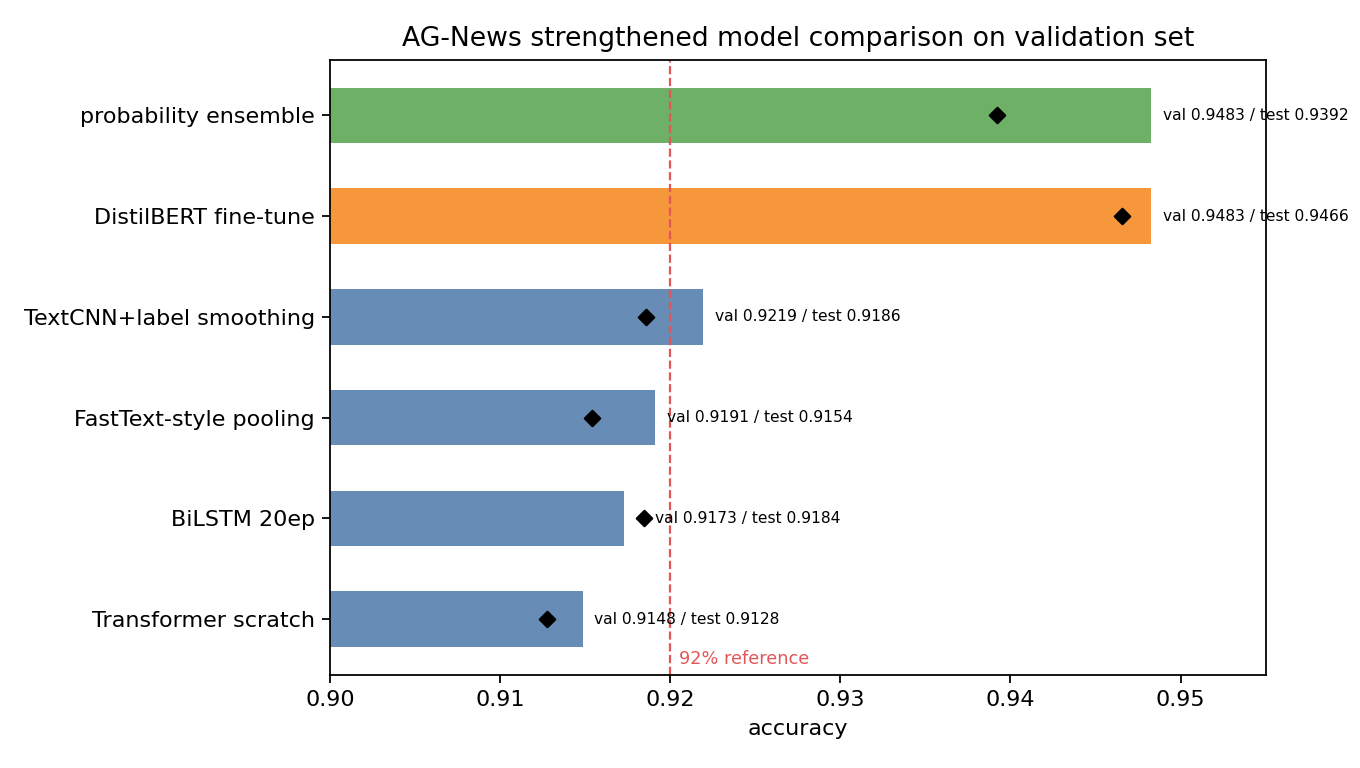
\includegraphics[width=0.9\textwidth]{ag_stage2_model_comparison.png}
\caption{AG-News strengthened model comparison on validation set. The axis is zoomed because all runs exceed 0.90 accuracy; black diamonds mark test accuracy.}
\end{figure}

该图将 scratch、pretrained 和 ensemble 用不同颜色区分，并同时标出 validation 与 test accuracy。它支持的结论是：DistilBERT 在 validation/test 上均领先，ensemble 已明显超过 92\% reference 但低于 DistilBERT 单模；scratch 模型集中在 0.915--0.922 validation 区间。

\begin{table}[H]
\centering
\caption{Best scratch model and pretrained model on AG-News}
\begin{tabular}{lccc}
\toprule
category & selected run & val acc & test acc \\
\midrule
Validation-selected scratch / lightweight & hparam\_dropout\_0.2 & 0.9228 & 0.9167 \\
Best scratch test observation & ag\_textcnn\_label\_smoothing & 0.9219 & 0.9186 \\
Pretrained fine-tuning & ag\_distilbert\_finetune & 0.9483 & 0.9466 \\
\bottomrule
\end{tabular}
\end{table}

它是说明引入大规模语料预训练表示后，AG-News 分类性能明显提升。scratch 模型内部仍按 validation set 做配置选择。

\section{AG-News 训练成本与泛化分析}
\begin{figure}[H]
\centering
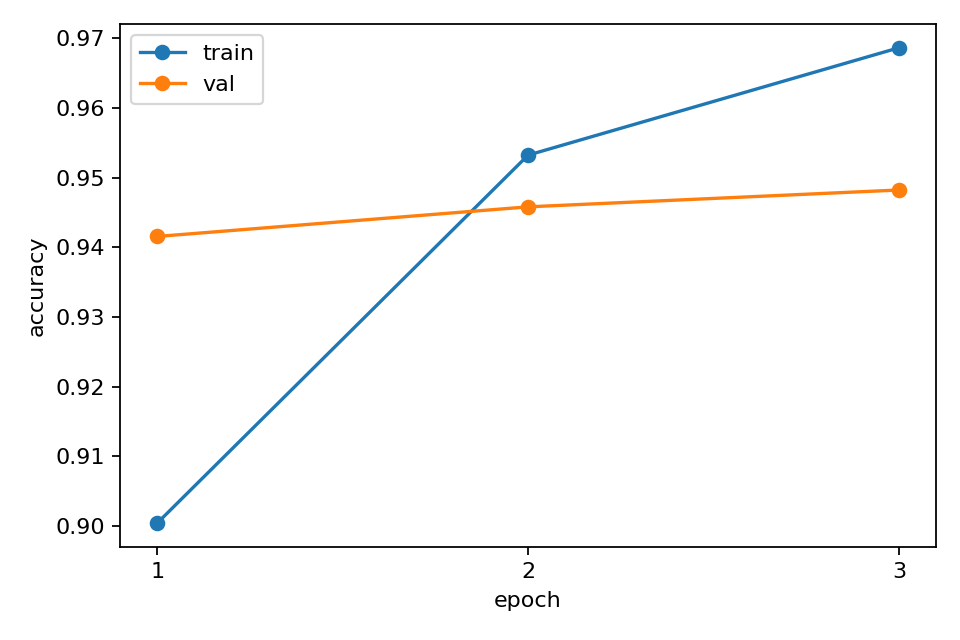
\includegraphics[width=0.72\textwidth]{ag_best_acc_curve.png}
\caption{DistilBERT train/validation accuracy curve}
\end{figure}

DistilBERT 的 validation accuracy 在 3 个 epoch 中从 0.9416 上升到 0.9483，best validation 出现在 epoch 3；train accuracy 同期从 0.9005 上升到 0.9687。该曲线说明预训练模型在短 fine-tuning 预算内快速适配 AG-News，但 train-validation 差距也在扩大。因此 3 epoch 是合理的核心实验预算：继续训练可能提高训练集拟合，却不保证 validation/test 同步提升。

\begin{table}[H]
\centering
\caption{AG-News representative training cost}
\small
\begin{tabular}{lrrrr}
\toprule
run & params & mean epoch time & total time & peak memory / test acc \\
\midrule
baseline\_textcnn & 4.04M & 10.3s & 61.6s & 162MB / 0.9149 \\
hparam\_dropout\_0.2 & 4.04M & 11.5s & 69.1s & 162MB / 0.9167 \\
ag\_textcnn\_label\_smoothing & 4.04M & 12.6s & 164.2s & 162MB / 0.9186 \\
ag\_rcnn & 4.20M & 48.4s & 532.1s & 289MB / 0.9117 \\
ag\_transformer\_encoder\_small & 5.99M & 66.8s & 869.0s & 798MB / 0.9128 \\
ag\_distilbert\_finetune & 66.96M & 402.9s & 1208.8s & 1713MB / 0.9466 \\
\bottomrule
\end{tabular}
\end{table}

训练成本表说明，TextCNN 系列在 8GB RTX 4060 Laptop 上属于低成本实验，单 epoch 约 10--13 秒；RCNN 和 scratch Transformer 明显更慢，但没有带来对应的 accuracy 改善。DistilBERT 的参数量和单 epoch 时间最高，不过 3 epoch 总时间仍在约 20 分钟量级，峰值显存 1713MB，符合本任务 24 小时复现实验预算。该表支持的结论是：成本增加本身不是充分条件，预训练表示迁移才是本轮 AG-News 性能跃升的主要原因。

\begin{figure}[H]
\centering
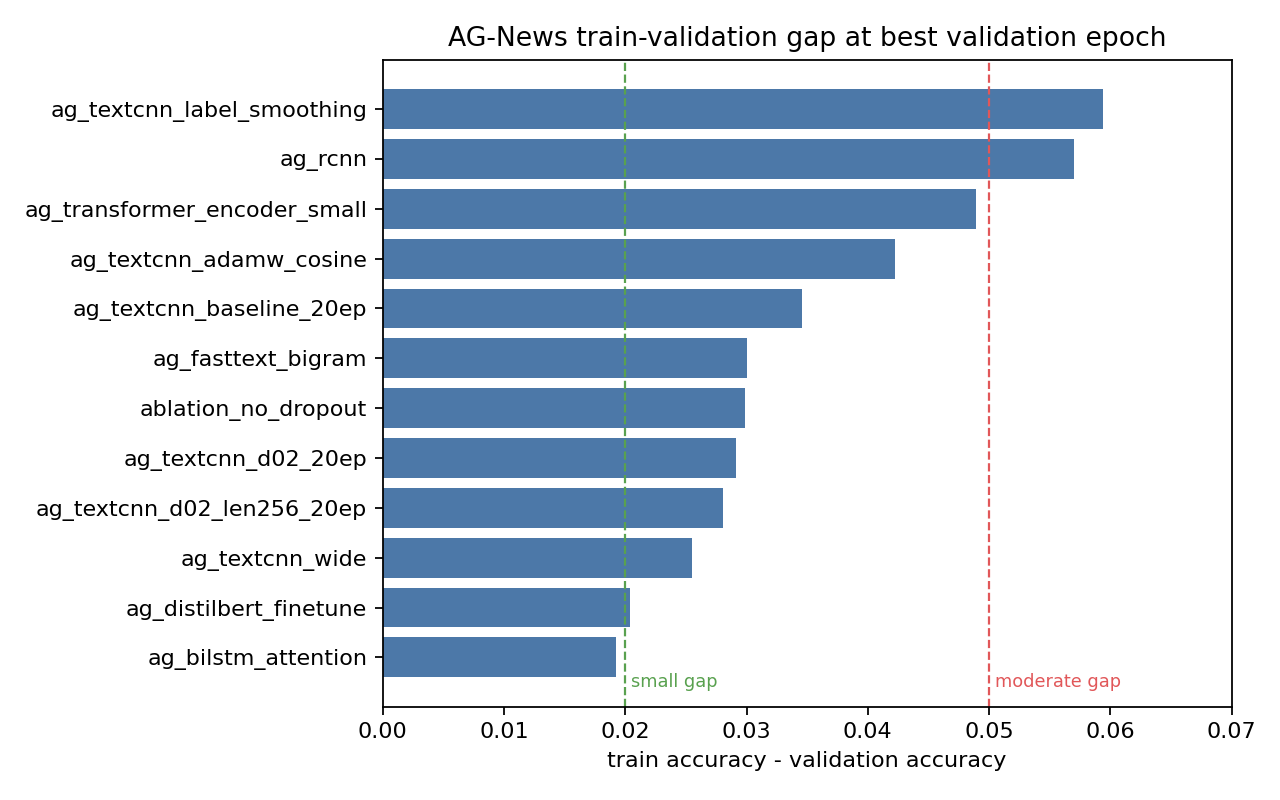
\includegraphics[width=0.72\textwidth]{ag_train_val_gap.png}
\caption{AG-News train-validation gap at best validation epoch}
\end{figure}

train-val gap 定义为 best validation epoch 上的 \(\mathrm{train\_acc}-\mathrm{val\_acc}\)。当前多数模型 gap 约 0.02--0.06，不能简单称为严重过拟合；更准确地说，部分模型出现轻度到中度 train-validation gap。较大的 gap 表明模型继续拟合训练集但验证集提升有限，较小的 gap 表明训练更稳定，但也可能意味着模型容量或训练预算不足。该图的价值不在于证明某个模型绝对过拟合，而在于与 test accuracy、模型容量、训练时间一起判断泛化行为。

\begin{figure}[H]
\centering
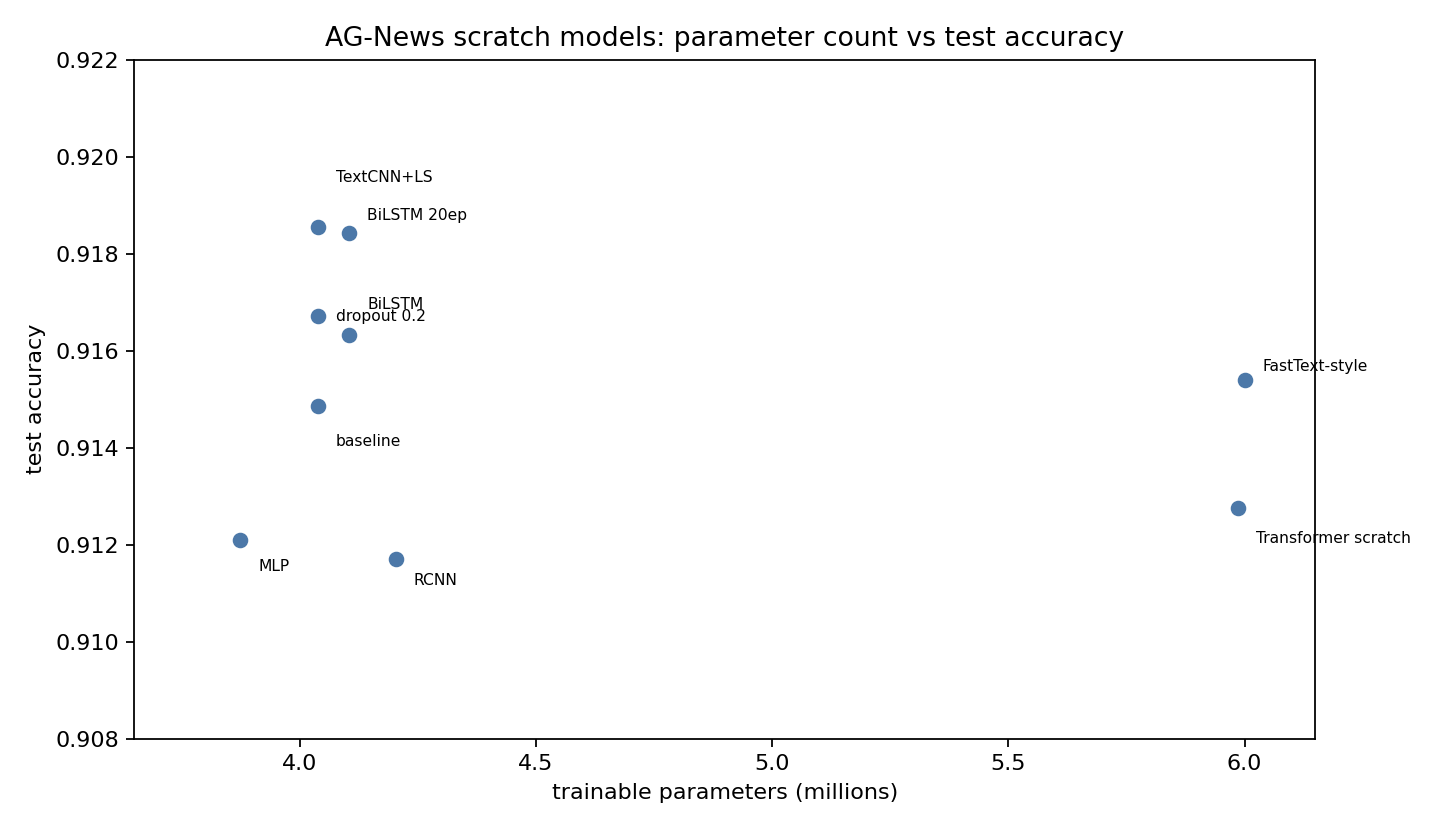
\includegraphics[width=0.72\textwidth]{ag_params_vs_accuracy.png}
\caption{AG-News scratch models: parameter count vs test accuracy. DistilBERT is excluded from this linear parameter-axis plot.}
\end{figure}

该图只比较 scratch / lightweight / strengthened non-pretrained 模型，避免 DistilBERT 约 66.96M 参数把线性横轴压缩到失去可读性。在 scratch 模型内部，参数量增加并不必然带来更高 test accuracy。例如 TransformerEncoder from scratch 参数量高于部分轻量模型，但没有超过 TextCNN，说明在 AG-News 上，预训练知识比简单扩大 scratch 模型更关键。DistilBERT 参数量约 66.96M，峰值显存约 1713MB，但它应作为预训练表示增强结果单独报告，不与 scratch 模型放在线性参数图中比较。

\section{AG-News 错误分析}
\begin{table}[H]
\centering
\caption{DistilBERT per-class metrics}
\begin{tabular}{lccc}
\toprule
class & precision & recall & F1 \\
\midrule
World & 0.9602 & 0.9532 & 0.9567 \\
Sports & 0.9879 & 0.9863 & 0.9871 \\
Business & 0.9252 & 0.9116 & 0.9183 \\
Sci/Tech & 0.9136 & 0.9353 & 0.9243 \\
\bottomrule
\end{tabular}
\end{table}

Sports 是最容易的类别，原因是实体、赛事和词汇边界清晰。Business 与 Sci/Tech 仍是主要难点，因为公司、产品、市场、软件和硬件新闻存在大量语义交叉。DistilBERT 明显降低了混淆，但没有消除这一边界问题。

\begin{figure}[H]
\centering
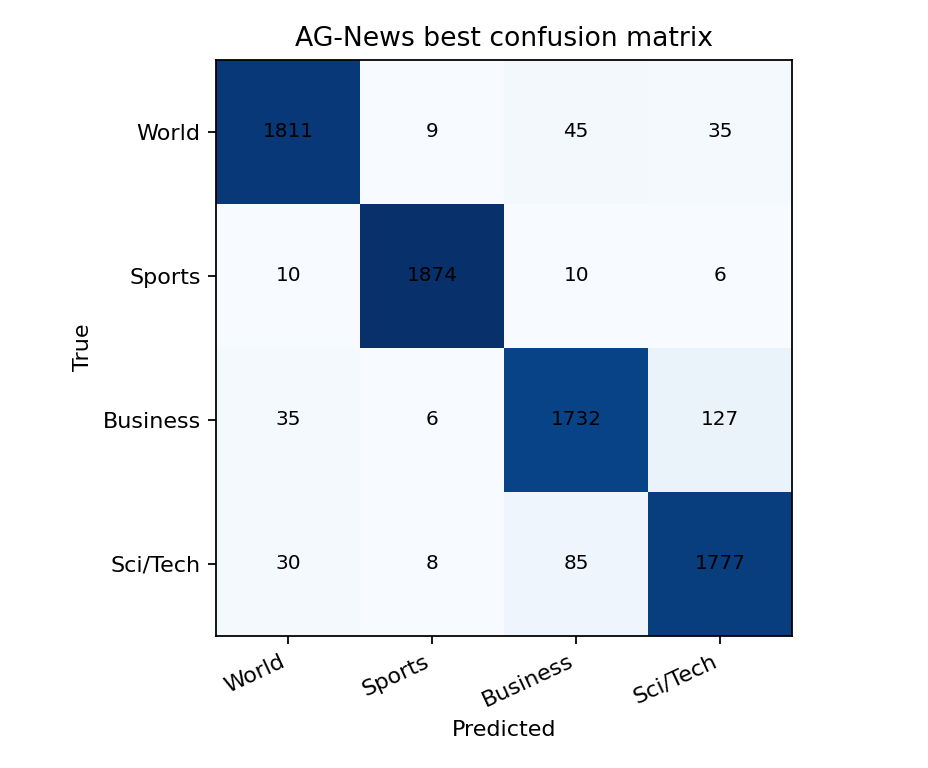
\includegraphics[width=0.62\textwidth]{ag_best_confusion_matrix.png}
\caption{AG-News best model confusion matrix}
\end{figure}

混淆矩阵显示 Sports 类最稳定，主要错误集中在 Business 与 Sci/Tech 的相互混淆。这支持了前文的类别解释：体育新闻实体和事件边界清晰，而商业、公司产品、技术发布和市场新闻存在语义重叠。该图只反映最终 DistilBERT 模型的错误分布，不应外推为所有模型的错误模式完全一致。

\begin{figure}[H]
\centering
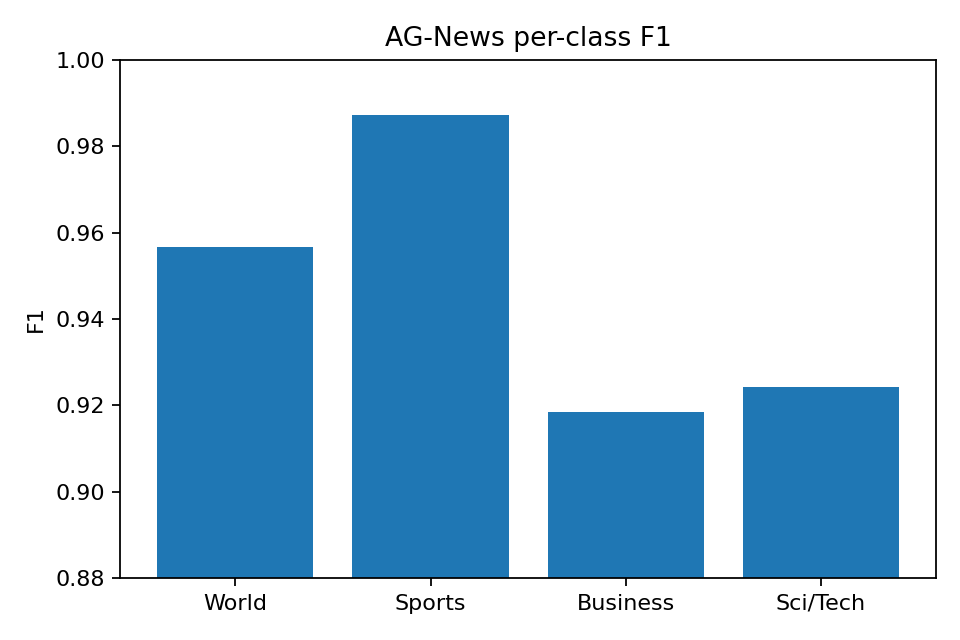
\includegraphics[width=0.62\textwidth]{ag_per_class_f1.png}
\caption{AG-News per-class F1}
\end{figure}

per-class F1 进一步说明类别难度不均衡：Sports 明显最高，Business 与 Sci/Tech 较低。由于 AG-News test split 每类样本数相同，这里的差异主要来自类别语义边界，而不是类别频率失衡。该图不能说明模型对所有 Business/Sci-Tech 样本都失败，只能说明这两个类别的平均边界更难。

\begin{figure}[H]
\centering
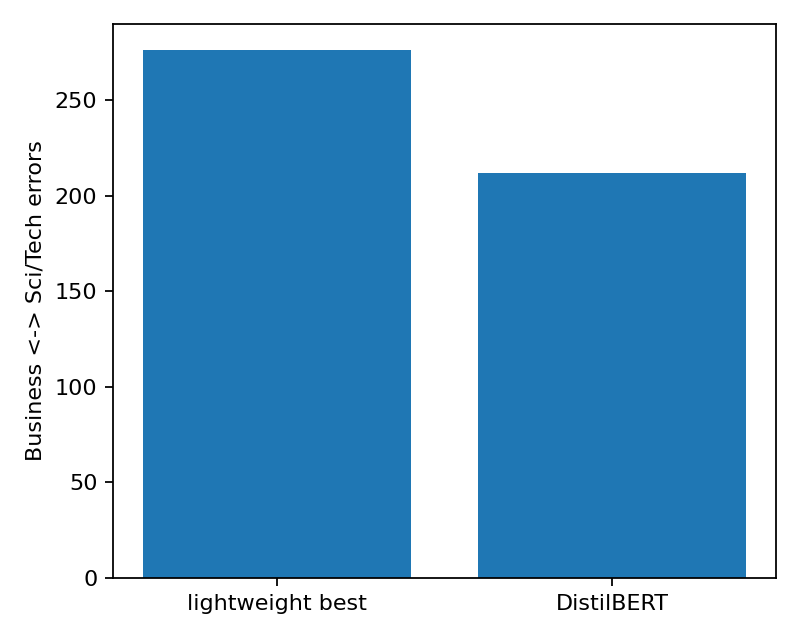
\includegraphics[width=0.62\textwidth]{ag_business_scitech_confusion.png}
\caption{Business/Sci-Tech confusion before and after pretraining}
\end{figure}

Business/Sci-Tech 专项图比较 lightweight best 与 DistilBERT 的互相混淆数量。DistilBERT 降低了该混淆，但没有完全消除，说明预训练上下文表示可以缓解语义边界问题，却不能把公司、产品、软件、市场这类天然交叉的新闻语义完全分开。

\section{结论与后续}
AG-News 方向最终选择 \texttt{ag\_distilbert\_finetune}，validation accuracy 为 0.9483，test observation accuracy 为 0.9466，超过 92\% 目标。scratch 文本模型提供了结构对比和错误来源解释，但未稳定突破 92\%。

\end{document}
